\section{Results} \label{sec:results}
% 1. Accuracy (F1 + MCC) auf SICK und eSNLI einzeln nach Kategorien
% 2. Auf Bias überprüfen: Vergleich vom Modell für wichtig erachtete Token mit von Menschen als wichitg erachtete Tokens
% Visualisierungen:
% - Confusion Matrix (Gentrennt nach Phänomenen)
% - Tabellen Interpretability Metriken (siehe ferret)

\paragraph{Detecting biases in data}
Figure~\ref{fig:metric-heatmap-phenomena-mcc} depicts the Matthews Correlation Coefficients for our model trained on different datasets separated by linguistic phenomena: \enquote{default} is the model trained on the regular \ac{MultiNLI} dataset, \enquote{filtered} trained on samples which where correctly classified of maximum two hypothesis only models and \enquote{hypothesis-only} is the model trained only on the hypotheses of \ac{MultiNLI}.

\begin{figure}[ht]
    \centering
    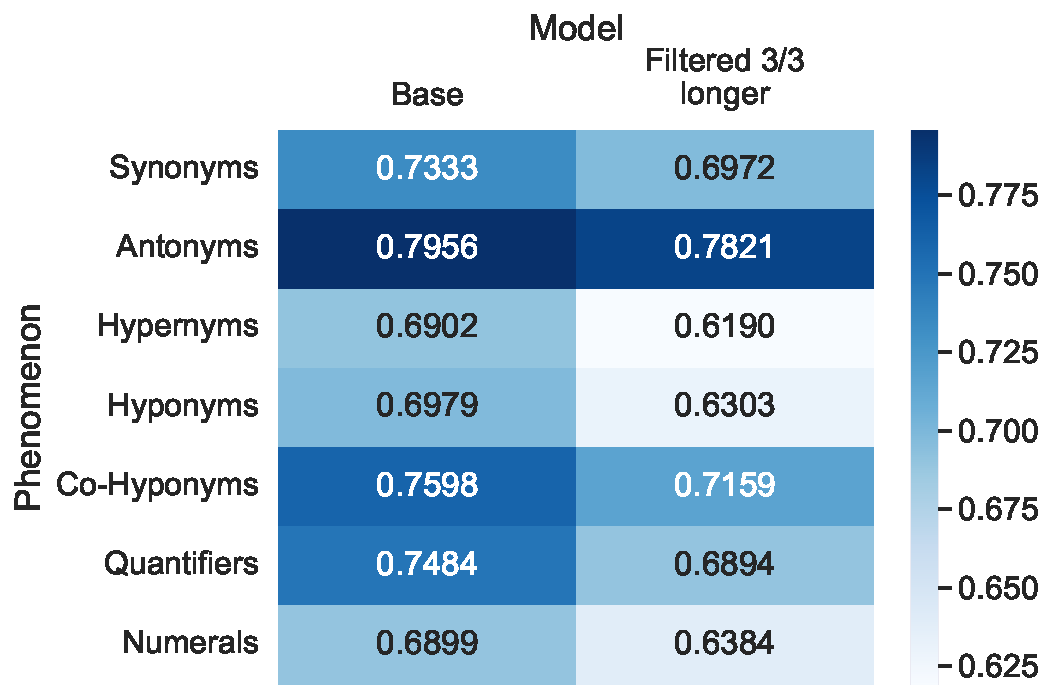
\includegraphics[width=0.9\columnwidth]{./images/metric_heatmaps_phenomena/important_words/matthews_correlation.pdf}
    \caption{Matthews Correlation Coefficients for the model trained on different datasets separated by linguistic phenomena}
    \label{fig:metric-heatmap-phenomena-mcc}
\end{figure}

The hypothesis-only model performs poorly as expected but also comparably well on samples that contain antonyms which indicates a bias in these samples and thus proves \textbf{H2}. The improved performance of the filtered model also shows that this bias can be mitigated by filtering the biased samples and thus proves \textbf{H4}.

The hypothesis-only model also performs better on samples that contain quantifiers which indicates a bias also in these samples. The filtered model performs slightly worse on quantifiers than the default model. Thus, it is not sufficient to filter out the biased samples to increase performance on quantifiers. A reason for this behavior might be the greater complexity of quantifiers compared to antonyms. To increase the model's performance on quantifiers nevertheless, we collect additional training samples containing quantifiers.

\begin{figure*}[h!]
    \centering
    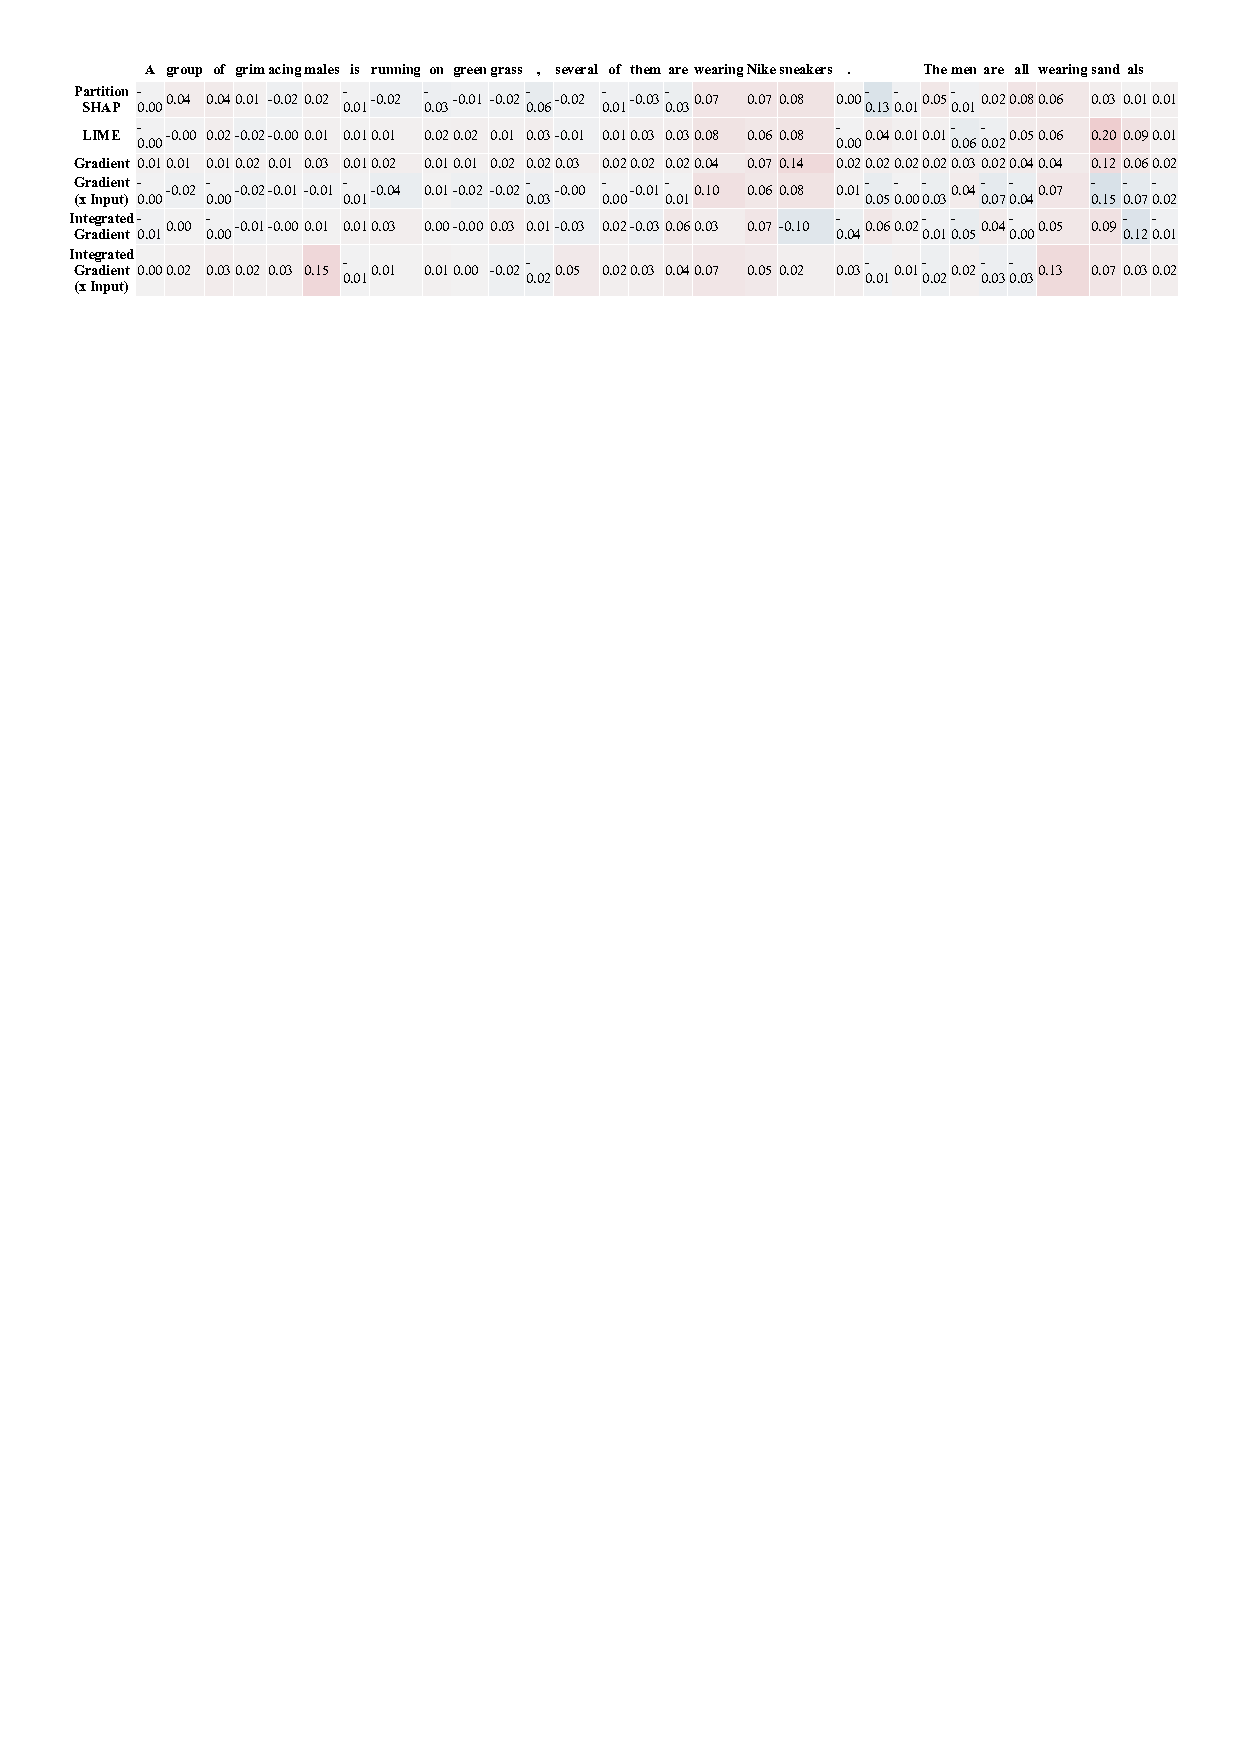
\includegraphics[width=\textwidth]{./images/ferret_sample.pdf}
    \caption{Expamle of a bad explanation}
    \label{fig:ferret-sample}
\end{figure*}

\FloatBarrier{}

\paragraph{Detecting biases in models}
Figure~\ref{fig:ferret-sample} shows the explanations for the default model's classification of a sample from the validation split of the \ac{e-SNLI} dataset obtained using ferret \cite{ferret}. It can be seen that the meaning of the quantifiers in this sample is not well captured by the model: The usage of quantifiers in this sample makes it a contradiction but the model only attaches comparably high importance to the quantifier \enquote{all} whereas \enquote{several} only has very low importance to the model. The existence of such samples where the model only poorly captures the importance of quantifiers proves \textbf{H2}.
